\chapter{Antecedentes}

% =====================================================================
% ESTRUCTURA OBJETIVO DEL CAP. 2 (tema NUEVO). NO BORRAR lo existente:
% 2.1 y 2.2 ya están cubiertos y se reusan casi tal cual.
%
%   2.1 LTS, autómatas y composición paralela.
%       -> YA ESTÁ: \subsection{Autómatas y composición paralela}.
%   2.2 Problema de control: safe y non-blocking.
%       -> YA ESTÁ: \subsection{Controlador}.
%   2.3 Síntesis composicional (Mohajerani-Malik-Fabian, Chalmers): la
%       noción de equivalencia que usa el paper composicional.
%       -> FALTA agregar. \cite{wsoe}, \cite{compositional}.
%
% Nota: la definición formal de WSOE se trasladó al Cap. 3, donde se
% define junto a branching bisimilarity y se demuestra su equivalencia.
% Su complejidad se contrasta con el O(m log n) del algoritmo de Groote
% et al. (Cap. 4).
%
% Nota: el \section{Un ejemplo concreto} (TravelAgency) más abajo apunta
% al benchmark, que en la estructura nueva es el Cap. 6.
% =====================================================================

En este capítulo agregaremos algunas definiciones y explicaciones necesarias para poder avanzar con la definición y análisis formal del problema composicional de síntesis de controladores.

\section{Definiciones utilizadas}

\subsection{Autómatas y composición paralela}
\noindent \textbf{Definición 1} (\textit{Autómata Determinístico}): Un autómata determinístico es una tupla $T = (S_{T}, A_{T}, \D_T, \init{t}, M_T)$, donde:  $S_T$ es un \k{conjunto finito de estados}, $A_T$ es un \k{conjunto finito de eventos del autómata}, $\D_T : S_T \x A_T  \rightarrow S_T$ es una \k{función de transición}, $\init{t} \in S_T$ es el \k{estado inicial del autómata} y $M_T \C S_T$ es el conjunto de \k{estados marcados}.

\noindent \textbf{Notación 1} (\textit{Pasos y corridas}): \ Notamos $(t,\l,t') {\in}\!\! \D_T$ como $t \step{\l}{T} t'$ y lo llamamos un \k{paso}.
A su vez, una \k{corrida} de una palabra $w = \l_0,\ldots,\l_k$ en $T$, es una secuencia de pasos tal que $t_i \step{\l_i}{T} t_{i+1}$ para todo $0 \leq i \leq k$, notado como $t_0 \runw{w}{T} t_{k+1}$.


\noindent \textbf{Notación 2}: \ Decimos que un estado $s$ es alcanzado por una palabra $w$ en una corrida comenzando en el estado $s'$, anotado como $s \in w(s')$, cuando $\exists w_{0} \ldot \exists w_{1} \ldot w = w_{0} \ldot w_{1}$ y $s' \runw{w_{0}}{E} s$.

\medskip

Los autómatas definen un lenguaje, un conjunto de palabras que aceptan. Dado un conjunto de eventos A, notamos con $A^{*}$ al conjunto de palabras finitas de eventos de A. El lenguaje generado por un autómata $T$, notado como $\L(T)$, es el conjunto de palabras formadas por eventos que cumplen $\D_T$. Formalmente, si $w \in A_T^*$, entonces $w \in \L(T)$ si y sólo si existe una corrida para $w$ comenzando desde el estado inicial  $\init{t}$ de $T$, que notamos $\init{t} \runw{w}{T} t'$. Generalmente los estados marcados se utilizan para indicar el logro de una tarea. Por lo tanto, consideramos como lenguaje marcado \textit{(o aceptado)} por $T$ (lo cual notamos $\L_m(T)$) al conjunto de palabras cuya corrida termina en un estado marcado.

Formalmente, sea $w \in \L(T)$, entonces $w \in \L_m(T)$ si y solo si hay una corrida de $w$ que comienza en el estado inicial $\init{t}$  y alcanza un estado marcado $t_m \in M_T$, que notamos $\init{t} \runw{w}{T} t_m$. Este último concepto es relevante para la definición de la composición paralela. Es una parte fundamental del trabajo para definir las palabras aceptadas por el problema \textit{nonblocking} ya que el lenguaje aceptado por la planta compuesta es el mismo que el aceptado por cada uno de los componentes por separado.

\medskip

\noindent \textbf{Definición 2} (\textit{Composición Paralela}): La composición paralela  $(\|)$ de dos autómatas $T$ y $Q$ es un operador simétrico y asociativo que produce un autómata \\ $T \| Q = (S_T 
{\times} S_Q, A_T {\cup} A_Q, \D_{T\|Q}, \<\init{t},\init{q}\>, M_T {\times} M_Q)$, donde $\D_{T\|Q}$ es la menor relación que satisface las siguientes reglas (omitimos la versión simétrica de la primera regla):

\begin{normalsize}
\centering
\vspace{-10pt}
\hspace{-50pt}
\begin{minipage}{0.30\linewidth}
\[ 
\frac{t \step{\l}{T} t'}{\<t,q\> {\step{\l}{T\|Q}} 
\<t'\!,\!q\> }{{\scriptstyle \l \in A_{T} {\setminus} 
A_{Q}}} 
\]
\end{minipage} 
\hspace{40pt}
\begin{minipage}{0.30\linewidth}
\[ 
\frac{t \step{\l}{T} t' \quad q \step{\l}{Q} 
q'}{\<t,q\> 
\step{\l}{T\|Q} \<t',q'\>}{{\scriptstyle \l \in A_{T} 
{\cap} A_{Q}}}
\]
\end{minipage} \\[15pt]
\end{normalsize}

Hay ciertas características de la composición paralela a destacar. En primer lugar, la última regla realiza la sincronización entre componentes. Segundo, que el número de estados en $T_0 \| \ldots T_n$ puede crecer exponencialmente con respecto al número de autómatas
a componer. Tercero, que el lenguaje aceptado por la composición contiene las palabras
que alcanzan estados marcados en todos los componentes simultáneamente.

\subsection{Controlador}

Dado un (conjunto de) autómata(s) y una partición de sus eventos en dos subconjuntos (controlables y no controlables), lo que buscamos es un \textit{controlador} que limite el vocabulario aceptado por el autómata de forma tal de mantener un camino posible a los estados marcados del mismo.


Un controlador observa las transiciones no controlables y puede deshabilitar algunas transiciones controlables para generar una planta restringida. Una palabra $w$ pertenece al lenguaje generado por $T$ restringido por una función del controlador $\sigma: A_T^* \into 2^{A_T}$ (anotado como $\L^\sigma(T)$) si cada prefijo de $w$ \textit{sobrevive} a $\sigma$. Formalmente, sea $w = \l_0, \ldots , \l_k$ una palabra en $\L(T)$, entonces $w \in \L^\sigma(T)$ si y solo si para todo $0 \leq i \leq k : \init{t} \runw{\l_0, \ldots , \l_i}{T} t_{i+1}  \wedge \l_i \in \sigma(\l_0, \ldots , \l_{i-1})$.

\noindent \textbf{Definición 3} (\textit{Problema de control \textbf{Safe} y \textbf{Non-Blocking}}): Un \textit{problema de control} con objetivos \textbf{Safe} y \textbf{Non-Blocking} composicional es una tupla $\E = (E, A_E^C, S_E^I)$, donde $E$ es un conjunto de autómatas $\{ E_0, \ldots, E_n\}$. En nuestro caso haremos un abuso de notación y usaremos $E =(S_E, A_E, \D_E, \init{e}, M_E)$ para referirnos a la composición $E_0 \| \ldots \| E_n$. Por otro lado, $A_E^C \subseteq  A_E$ es el conjunto de eventos controlables y definimos analogamente a $A_E^{U} = A_E \setminus A_E^{C}$ como el conjunto de eventos \textbf{no} controlables.

Una solución para $\E$ es un supervisor $\sigma : A_E^* \into 2^{A_E}$, tal que $\sigma$ es:

\begin{itemize}
    \item \textit{Controlable}: $A_E^{U} \subseteq \sigma(w)$ con $w \in A_E^{*}$
    \item \textit{Safe y non-blocking}: para cada palabra $w \in \L^\sigma(E)$ existe una palabra no vacía $w' \in A_E^*$ tal que la concatenación $ww' \in \L^\sigma(E)$ y $\init{e} \runw{ww'}{E} e_m$ con $e_m \in M_E$ (un estado marcado de E).
\end{itemize}

Por lo tanto concluímos que un supervisor $\sigma$ es \textit{controlable} si deshabilita solamente eventos controlables, y es \textit{safe y non-blocking} si podemos garantizar para cualquier palabra del lenguaje una extensión que le permita llegar a un estado marcado. A continuación definiremos como \textit{ganadores} (\textit{perdedores}) a los estados que podemos (no podemos) incluir en un controlador.

Decimos que un estado $s$ es \textbf{ganador} en el problema $\E = (E, A_E^C, S_E^I)$ si hay una solución $(E_s, A_E^{C})$ donde $E_s$ es el resultado de cambiar al estado inicial de $E$ a $s$.

Podemos pensar en un controlador \textit{non-blocking} como un jugador optimista que se encarga de no perder, y solo requiere conocer un futuro camino posible para llegar a un estado ganador. Es importante notar que como se busca que cualquier palabra sea extensible a otro estado marcado, lo que se busca es pasar por algún estado marcado infinitas veces. Es
decir, un estado \textit{e} marcado que tenga un camino para que el jugador pueda volver \textit{controlablemente} al mismo estado \textit{e}.

Por esto es que a lo largo de este trabajo analizaremos detenidamente la estructura de ciclo en nuestro algoritmo ya que sirve para deducir propiedades como que los primeros estados ganadores son aquellos que están en un loop controlable con un estado marcado dentro. Luego anotamos como ganador también a cualquier estado que controlablemente alcanza un estado ganador.

Los ciclos también son esenciales para encontrar los estados perdedores, ya que la única forma de que un estado sea perdedor es que no pueda alcanzar un estado ganador. En otras palabras, los estados perdedores son aquellos que forman parte de un loop que no tiene estados marcados ni transiciones salientes, asímismo los que llevan a un deadlock.


% =====================================================================
% TODO(2.3): \section{Síntesis composicional} -- AGREGAR.
%   - Marco de Mohajerani / Malik / Fabian (Chalmers): minimización entre
%     composiciones para evitar la explosión de estados. \cite{wsoe}.
%   - Cuál es la noción de equivalencia que habilita esa minimización y
%     cómo la usa el paper composicional. \cite{compositional}.
%
% NOTA DE REORGANIZACIÓN: la definición formal de WSOE (antes planificada
% acá como §2.4) se movió al Cap. 3 (Branching bisimilarity), donde se
% define junto a branching y se demuestra su equivalencia.
% =====================================================================

\section{Un ejemplo concreto}

Para ejemplificar y tener una noción acerca del tamaño que puede alcanzar el problema de composición y su posterior exploración, presentaremos una versión simplificada del problema \textbf{TravelAgency} que describiremos con mayor detalle posteriormente en el capítulo 6 y será usado para medir la \textit{performance} del algoritmo.

En este problema se busca armar una agencia de venta online de paquetes vacacionales. El objetivo
es que la misma orqueste los servicios (alquiler de auto, hotel, pasaje de avión, etc.) de forma automática de manera de obtener un paquete de vacaciones completo de ser posible, evitando pagar por paquetes incompletos.

Para cada servicio que se desea sub-contratar se consulta (query) si ese servicio está disponible. En caso de tener éxito y confirmar la disponibilidad, se espera a confirmar el resto para comprar todos al mismo tiempo. En caso de que algún otro servicio no esté disponible, se cancela la compra y se vuelve al estado inicial, lo cual no implica un gasto.

Este problema, descripto por ahora en términos generales, puede escalar de forma muy rápida si se incrementa la cantidad de servicios a contratar o la cantidad de pasos para reservar cada servicio,
por lo que para este ejemplo ilustrativo asumimos que no hacen falta múltiples pasos para reservar un servicio, y solo mostramos el problema con 1 y 2 sub-servicios.

\begin{figure}[h!]
    \centering
    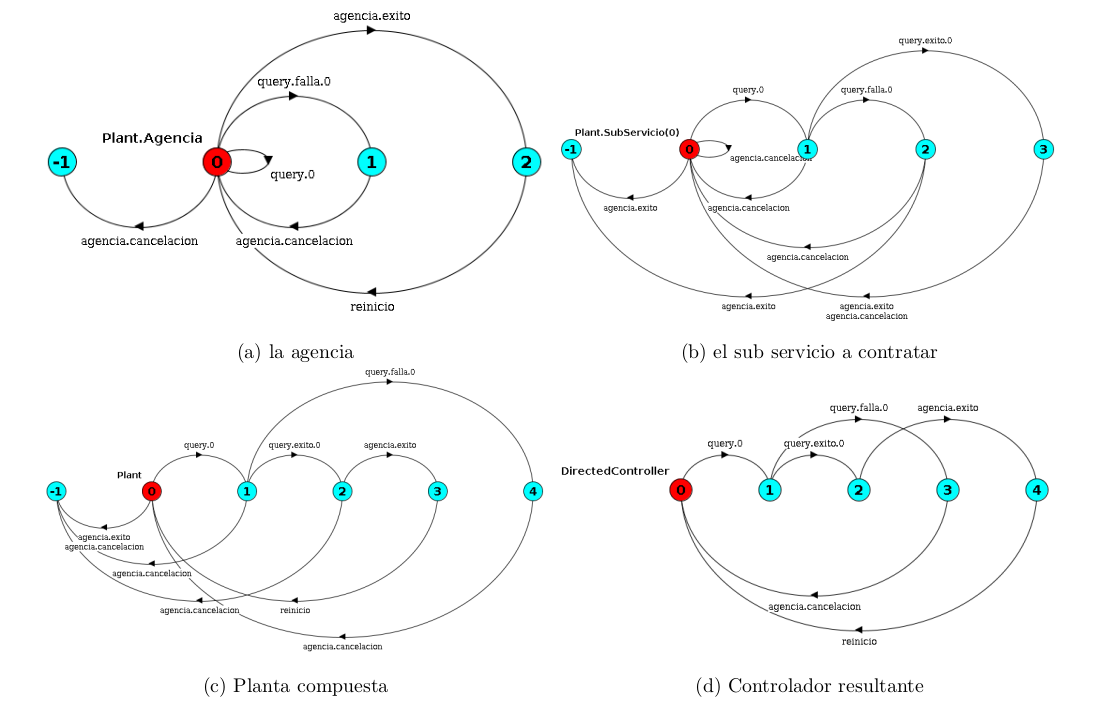
\includegraphics[width=1\textwidth]{capitulos/cap1/img/TAEjemploMTSA.png}
    \caption{Ejemplo del problema Travel Agency (TA) con un solo sub-servicio}
    \label{fig:ejemploTAProblema}
\end{figure}

En el ejemplo, la figura \ref{fig:ejemploTAProblema}a es la representación de la agencia que busca confirmar la compra, el estado 2 es nuestro estado marcado, objetivo que queremos alcanzar infinitas veces. En cambio, al detectar algún \textit{query.falla}, se mueve al estado 1, señalando que hubo un problema y solo permite cancelar la compra de todos los otros servicios consultados.

El componente del \textit{subservicio} (figura \ref{fig:ejemploTAProblema}b) también tiene el evento \textit{agencia.exito}, pero debe previamente haber recibido la consulta y confirmado su disponibilidad tomando el evento \textit{query.exito.0}. 

En caso de no ser posible la reserva, solo permite la cancelación de la compra, yendo del estado 2 al 0; si se
quisiera confirmar la compra (\textit{agencia.exito}) se llega al \textbf{estado -1}, reservado para los errores
que el controlador debe evitar.

Podemos observar la representación del sistema complejo en la sincronización que se ve reflejada en la figura \ref{fig:ejemploTAProblema}c, que muestra la planta que representa al sistema con los dos componentes previamente descriptos.

Finalmente, \ref{fig:ejemploTAProblema}d muestra un posible controlador para este problema. Destacamos que todos los eventos controlables que llevaban al estado -1 (el estado error), no son una posibilidad permitida por el controlador.

\begin{figure}[h!]
    \centering
    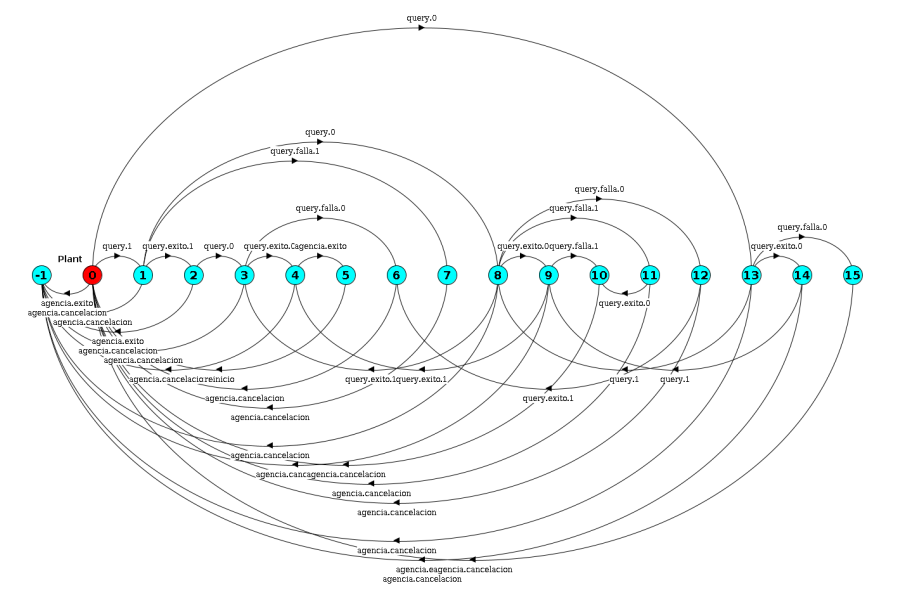
\includegraphics[width=.85\textwidth]{capitulos/cap1/img/EjemploTACompuestoMTSA.png}
    \caption{Planta compuesta para 2 sub-servicios}
    \label{fig:ejemploTAPlanta}
\end{figure}

\FloatBarrier

Si analizamos el tamaño que adquiere la planta compuesta expresada en la figura \ref{fig:ejemploTAPlanta} podemos notar que es un tipo de problema que escala rápidamente cuando se incrementan los autómatas que se van a componer. También podemos ver que el controlador posee un subconjunto de estados y transiciones de la planta compuesta total. 

Por esta razón reafirmamos el enfoque de exploración \textit{on-the-fly} para resolver el problema de síntesis evitando, en la medida de lo posible, la composición de todo el modelo. 

\vspace{5cm}

